\documentclass[conference]{IEEEtran}

\usepackage{amsmath,amssymb}
\usepackage{booktabs}
\usepackage{cite}
\usepackage{graphicx}
\usepackage[hidelinks]{hyperref}
\usepackage{xcolor}

\graphicspath{{../paper_assets/}}
\definecolor{todoRed}{RGB}{170,35,35}
\newcommand{\todo}[1]{\textcolor{todoRed}{\textbf{[[TODO: #1]]}}}
\newcommand{\method}{REIM}
\newcommand{\risk}{p_t}
\newcommand{\noise}{\lambda}

\setlength{\textfloatsep}{7pt plus 2pt minus 2pt}
\setlength{\floatsep}{6pt plus 2pt minus 2pt}
\setlength{\intextsep}{6pt plus 2pt minus 2pt}
\setlength{\abovecaptionskip}{4pt}
\setlength{\belowcaptionskip}{0pt}

\title{Recovery-Enhanced Imitation Learning for\\
Robust Multi-Task Robot Manipulation}

\author{
\IEEEauthorblockN{\todo{replace with verified author names}}
\IEEEauthorblockA{\todo{replace with affiliations and contact email}}
}

\begin{document}
\maketitle

\begin{abstract}
Action-chunking policies can execute long, smooth manipulation sequences, but a small state or action deviation may move the robot outside the distribution represented by the current chunk. We present Recovery-Enhanced Imitation Learning (REIM), a runtime wrapper that combines a task-conditioned Action Chunking with Transformers policy, a causal LSTM risk monitor, and a task-conditioned recovery policy through hysteretic control arbitration. The monitor is trained on future behavioral-deviation events, while recovery supervision is collected from successful expert continuations at online trigger states. We evaluate separately trained models on the known-task, goal-observable Meta-World MT10 and MT50 suites. The clean protocol and a paired Gaussian-perturbation extension each use 50 episodes per task. At the strongest tested perturbation, REIM attains 63.0\% task-macro success on MT10 and 49.52\% on MT50, compared with 46.4\% and 33.96\% for the same learned recovery policy under a reward-stagnation gate. Clean success remains 97.6\% and 92.24\%, respectively. Paired outcomes and per-task analysis show that recovery is beneficial on most, but not all, task families; high intervention occupancy under strong perturbations remains an important limitation.
\end{abstract}

\begin{IEEEkeywords}
robot learning, imitation learning, recovery policy, runtime monitoring, multi-task manipulation
\end{IEEEkeywords}

\section{Introduction}
\label{sec:introduction}

Imitation learning can produce effective manipulation controllers without an explicit dynamics model, yet closed-loop deployment remains sensitive to covariate shift. A small execution error changes the next observation, which changes the next prediction, and the resulting state sequence may progressively depart from the demonstrations. Action chunking reduces high-frequency action inconsistency by predicting temporally extended commands, but it does not by itself decide when the nominal policy should stop controlling the robot. This distinction matters in long-horizon manipulation: continuing a locally inappropriate chunk can convert a recoverable deviation into a task failure.

Existing recovery systems often assume either a hand-designed trigger, an external safety signal, or a separate reinforcement-learning objective. These choices complicate a fair diagnosis of where improvement comes from. A recovery policy may be competent while its trigger is late; conversely, an aggressive trigger may invoke recovery almost continuously and harm nominal states. The central problem is therefore not only how to learn recovery actions, but how to arbitrate between nominal and recovery control using causal information available at runtime.

We introduce Recovery-Enhanced Imitation Learning (REIM), a supervised recovery architecture for known-task multi-task manipulation. As illustrated in Fig.~\ref{fig:overview}, a task-conditioned ACT policy supplies nominal action chunks, an LSTM consumes the most recent state history and estimates near-term behavioral-deviation risk, and a task-conditioned multilayer perceptron supplies recovery actions. A hysteretic state machine turns the continuous risk estimate into stable control decisions. Separate entry and release conditions prevent rapid switching, a minimum dwell time gives recovery an opportunity to act, and a cooldown period prevents immediate retriggering.

The risk target is not terminal task success. Instead, it identifies whether a task-calibrated disagreement event will occur in the immediate future. Consequently, detector precision and end-to-end task success are different quantities: a monitor with moderate classification precision can still be useful when its mistakes are filtered by hysteresis and the downstream policy is trained on the states where intervention actually occurs. We evaluate this system on MT10 and MT50 with task identity exposed, following the goal-observable use of these suites. The two suites share the same disturbance definition and evaluation logic but use separately trained models; their absolute scores are therefore compared as evidence of scaling behavior, not as samples from one pooled policy.

This work makes three contributions:
\begin{itemize}
  \item a causal, task-conditioned risk monitor with validation-only operating-point selection and explicit hysteretic arbitration;
  \item a trigger-aligned supervised recovery dataset constructed from successful expert continuations at policy-induced states; and
  \item a paired evaluation across MT10 and MT50 that reports clean performance, a common perturbation sweep, rescued and harmed episodes, and per-task heterogeneity.
\end{itemize}
We deliberately avoid a state-of-the-art claim. The evidence supports robustness under the tested simulation protocol; it does not establish unseen-task generalization, calibrated failure probabilities, or real-robot reliability.

\begin{figure*}[t]
  \centering
  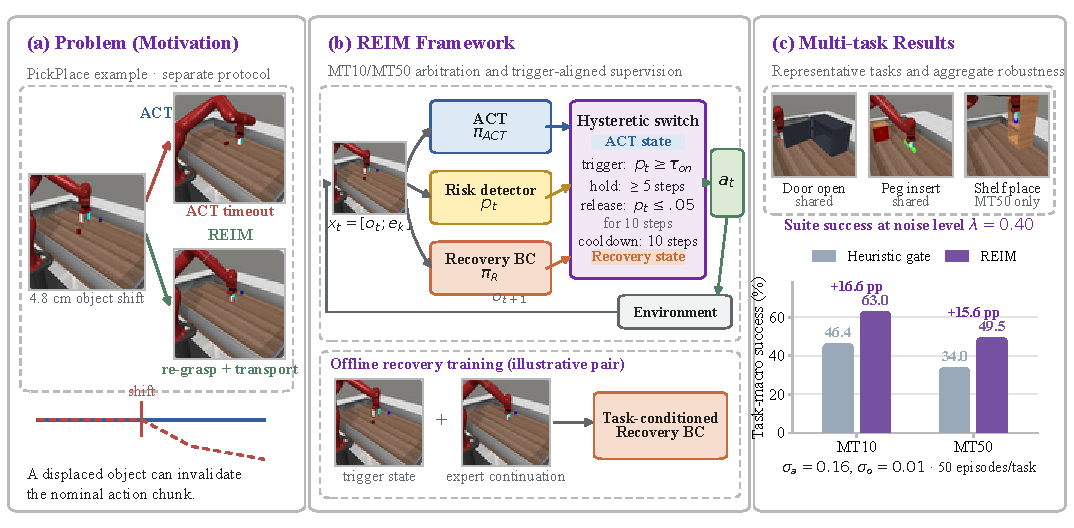
\includegraphics[width=\textwidth]{Figure1_v12_overview.pdf}
  \caption{REIM overview. (a) A separate PickPlace example motivates recovery after ACT drift. (b) Task-conditioned nominal control, causal risk monitoring, and hysteretic arbitration. (c) Representative MT tasks and headline results at $\noise=0.40$; MT10 and MT50 models are trained separately.}
  \label{fig:overview}
\end{figure*}

\section{Related Work}
\label{sec:related}

\subsection{Imitation Learning and Action Chunking}
Behavioral cloning directly fits expert state--action pairs but can accumulate errors when the learned policy visits states absent from the demonstrations. Dataset aggregation addresses this mismatch by querying an expert at states induced by the learner~\cite{ross2011dagger}. ACT instead predicts fixed-length action chunks with a conditional variational Transformer and temporally ensembles overlapping predictions~\cite{zhao2023act}. REIM uses ACT as the nominal controller. Its recovery collection is related to dataset aggregation because supervision is obtained at policy-induced trigger states, although the present pipeline does not iteratively retrain the nominal policy.

\subsection{Runtime Monitoring and Recovery}
Runtime monitors can detect inconsistency or stalled progress without changing the base policy~\cite{agia2025sentinel}. Learned recovery has also been studied through safe reinforcement learning, residual control, meta-reasoning, and local policy chaining~\cite{thananjeyan2021recovery,johannink2019residual,vats2023metareskill,vats2024recoverychaining}. REIM differs in scope: both the recovery policy and the risk monitor are trained by supervised learning, and the learned gate is compared with a reward-stagnation gate while holding the recovery policy fixed. This isolates the contribution of arbitration from the existence of a recovery controller.

\section{Method}
\label{sec:method}

\subsection{Problem Formulation}
Consider a manipulation suite with $K$ known tasks. At step $t$, the environment provides a 39-dimensional state observation $o_t$ and task identity $k$. We concatenate the state with a one-hot task code,
\begin{equation}
  x_t=[o_t; e_k]\in\mathbb{R}^{39+K},
\end{equation}
so MT10 and MT50 use 49- and 89-dimensional policy inputs. An episode succeeds when the environment's official success signal is observed within 500 steps. REIM combines a nominal policy $\pi_N$, risk monitor $D$, recovery policy $\pi_R$, and arbitration state $z_t\in\{N,R\}$.

\subsection{Nominal Multi-Task ACT}
The nominal controller is a state-based ACT policy~\cite{zhao2023act}. Given $x_t$, it predicts a chunk of 20 four-dimensional actions. Training minimizes an $\ell_1$ reconstruction loss plus the ACT latent KL term. Overlapping predictions are combined using exponential temporal ensembling. We train distinct ACT models for MT10 and MT50 because the task vocabularies and input dimensions differ. Both use three encoder layers, four decoder layers, eight attention heads, and KL weight 10; hidden/latent dimensions are 256/32 for MT10 and 384/48 for MT50.

\subsection{Causal Near-Term Risk Monitor}
The monitor receives only the latest $L=10$ conditioned states. A one-layer LSTM maps $x_{t-L+1:t}$ to a hidden representation, followed by a two-layer classifier and sigmoid output
\begin{equation}
  \risk=\sigma\!\left(D(x_{t-L+1:t})\right).
\end{equation}
Because no future observation is used at inference, the monitor is causal.

Risk labels are derived from action disagreement rather than terminal success alone. For each task, the 90th percentile of $\ell_1$ disagreement between ACT and the scripted expert is fitted on the failure-training bank. A step is a risk event when its disagreement reaches that task-specific threshold. Failed rollouts also mark their final 25 steps as events. The binary target at time $t$ is positive if an event occurs within the next 10 steps. Task thresholds fitted on the training bank are frozen for validation and final evaluation.

The detector is optimized with weighted binary cross entropy. Deployment thresholds are selected only on the independent validation bank subject to task-macro precision of at least 0.60; the selected operating points are $\tau_{\mathrm{on}}=0.65$ for MT10 and $0.64$ for MT50. These validation metrics are not task success rates and should not be read as such.

\subsection{Trigger-Aligned Recovery Policy}
Recovery data are collected by running the nominal ACT policy and monitoring risk online. A deliberately broad collection threshold of 0.20 captures candidate recovery starts. Once triggered, a scripted task expert controls the continuation. Only successful continuations are retained, yielding 50 trigger-aligned trajectories per task. This creates recovery supervision at states encountered by the learned nominal controller rather than only at states from clean demonstrations.

The recovery controller is a deterministic task-conditioned MLP with hidden dimensions $512$--$512$--$256$ and Tanh activations. It is trained with Smooth-$\ell_1$ action loss, state noise augmentation of standard deviation 0.005, and task-balanced sampling. MT10 contains 500 recovery trajectories (30,807 training and 7,973 validation steps); MT50 contains 2,500 trajectories (159,581 training and 39,746 validation steps). As with ACT, a separate recovery model is trained for each suite.

\subsection{Hysteretic Control Arbitration}
The controller enters recovery when $\risk\geq\tau_{\mathrm{on}}$ and no cooldown is active. It remains in recovery for at least five steps. Thereafter, it releases control only after $\risk\leq0.05$ for ten consecutive steps. A ten-step cooldown follows release, and a single intervention is capped at 250 recovery steps. Formally, the principal transitions are
\begin{align}
 z_t=N &\rightarrow R &&\text{if } \risk\geq\tau_{\mathrm{on}} \text{ and cooldown}=0,\\
 z_t=R &\rightarrow N &&\text{if } n_R\geq5 \text{ and } n_{\mathrm{safe}}\geq10.
\end{align}
The thresholds implement hysteresis: evidence required to enter recovery is intentionally much stronger than evidence required to remain nominal after a sustained safe period. ACT's temporal state is reset whenever control returns from recovery.

\subsection{Why Collection and Deployment Thresholds Differ}
The recovery collection threshold and deployment threshold serve different statistical purposes. During collection, the objective is coverage: the recovery learner should see a broad range of states near the boundary of nominal behavior. A lower threshold of 0.20 therefore favors recall and lets the expert demonstrate how to continue before a deviation becomes terminal. At deployment, the objective is control selection: an unnecessary switch can interrupt a successful ACT chunk. The higher suite-specific thresholds are consequently chosen under a precision constraint. This separation is fixed before final evaluation and should not be interpreted as tuning the recovery policy on test outcomes.

The same distinction explains why the monitor is trained on near-term deviation rather than episode-level failure. A terminal label assigns one outcome to hundreds of preceding states, many of which may be nominal, and gives little temporal guidance about when to switch. The event target localizes supervision around task-relative disagreement and propagates it only ten steps backward. The resulting score is an operational ranking signal. Hysteresis then converts that signal into a decision using temporal persistence rather than assuming that each score is a calibrated failure probability.

\section{Experimental Protocol}
\label{sec:protocol}

\subsection{Benchmarks and Data Separation}
We use Meta-World 3.1.1~\cite{yu2020metaworld} with MuJoCo~\cite{todorov2012mujoco}. MT10 and MT50 provide 10 and 50 manipulation task families with known task identities. We use the goal-observable state representation and the official 500-step horizon. For each suite, task variants are reserved in distinct banks for demonstrations, detector training, recovery training, detector validation, and final evaluation. A digest-based audit verifies that the materialized task payloads and sampling-unit identities are disjoint across these stages.

Each task contributes 50 expert demonstrations, 50 failure-training rollouts, 50 retained recovery continuations, and 20 detector-validation rollouts. Final results use a separate confirmation bank with 50 episodes per task: 500 paired episodes per method for MT10 and 2,500 for MT50. Task variants, episode seeds, and injected noise arrays are shared across methods within a condition. No data from the confirmation bank are used to train a model or select a threshold.

Table~\ref{tab:scale} summarizes the scale of the two independently trained suites. The counts are deliberately symmetric per task; MT50 increases coverage by adding task families rather than by allocating fewer samples to each family. This design makes the MT10/MT50 comparison informative about breadth while avoiding a sample-budget confound at the task level.

\begin{table}[t]
\centering
\caption{Suite construction and final evaluation scale.}
\label{tab:scale}
\footnotesize
\setlength{\tabcolsep}{4.0pt}
\begin{tabular}{lrr}
\toprule
Quantity & MT10 & MT50 \\
\midrule
Task families & 10 & 50 \\
Conditioned state dimension & 49 & 89 \\
Expert demonstrations & 500 & 2,500 \\
Failure-training rollouts & 500 & 2,500 \\
Recovery continuations & 500 & 2,500 \\
Detector-validation rollouts & 200 & 1,000 \\
Episodes/method/condition & 500 & 2,500 \\
Final task-macro units & 10 & 50 \\
\bottomrule
\end{tabular}
\end{table}

\subsection{Methods Compared}
We compare four controllers. \emph{MT-MLP BC} is a two-layer $256$--$256$ behavioral-cloning policy. \emph{MT-ACT} is the nominal action-chunking controller. \emph{Heuristic+recovery} uses the same learned recovery policy as REIM but triggers when reward variation over a 20-step window falls below 0.01 after step 30. \emph{REIM} replaces this heuristic with the learned risk monitor and hysteretic state machine. Holding $\pi_R$ fixed between the last two methods makes their difference an arbitration comparison.

Table~\ref{tab:gate} summarizes the validation-selected detector operating points and the controller settings frozen before confirmation evaluation. The precision, recall, and expected calibration error (ECE) entries characterize near-term risk-event classification on the validation bank; they are not task-success metrics.

\begin{table}[t]
\centering
\caption{Validated detector operating points and frozen control settings.}
\label{tab:gate}
\footnotesize
\setlength{\tabcolsep}{3.0pt}
\begin{tabular}{lcc}
\toprule
Quantity & MT10 & MT50 \\
\midrule
Trigger threshold & 0.65 & 0.64 \\
Task-macro precision & 0.600 & 0.600 \\
Task-macro recall & 0.505 & 0.535 \\
Task-macro ECE & 0.138 & 0.141 \\
\midrule
Release threshold & 0.05 & 0.05 \\
Release patience (steps) & 10 & 10 \\
Minimum recovery (steps) & 5 & 5 \\
Cooldown (steps) & 10 & 10 \\
Recovery budget (steps) & 250 & 250 \\
\bottomrule
\end{tabular}
\end{table}

\subsection{Clean and Perturbed Evaluation}
Official-clean evaluation uses unmodified benchmark execution. Robustness is evaluated separately with task-universal independent Gaussian noise. For level $\noise$,
\begin{equation}
 \epsilon^a_t\sim\mathcal{N}(0,(0.4\noise)^2I_4),\qquad
 \epsilon^o_t\sim\mathcal{N}(0,(0.025\noise)^2I_{39}),
\end{equation}
with $\noise\in\{0,0.10,0.20,0.30,0.40\}$. Actions are clipped to the environment range after perturbation. Object positions are never teleported in this multi-task protocol. At $\noise=0.40$, the action and observation standard deviations are 0.16 and 0.01. This sweep is a REIM robustness extension, not an official Meta-World score.

The primary metric is task-macro success: success is averaged within each task and then equally across tasks. We report 95\% within-task episode-bootstrap intervals using 5,000 bootstrap samples. Paired rescued and harmed counts use the same task variant, episode seed, and noise realization for the two compared methods. Recovery occupancy is the fraction of executed steps controlled by $\pi_R$.

For paired comparison against the heuristic gate, let $s_i^R$ and $s_i^H$ be binary outcomes for matched episode $i$. We report rescued episodes when $(s_i^R,s_i^H)=(1,0)$ and harmed episodes when $(s_i^R,s_i^H)=(0,1)$. Their normalized difference equals the paired success-rate change,
\begin{equation}
 \Delta_{R-H}=\frac{1}{N}\sum_{i=1}^{N}(s_i^R-s_i^H)
 =\frac{N_{\mathrm{rescued}}-N_{\mathrm{harmed}}}{N}.
\end{equation}
This decomposition retains the direction of every discordant episode and prevents an aggregate improvement from being mistaken for uniform benefit.

\section{Results}
\label{sec:results}

\subsection{Clean Performance Is Largely Preserved}
At $\noise=0$, MT-ACT obtains 97.4\% success on MT10 and 91.64\% on MT50. REIM obtains 97.6\% [96.2, 98.8] and 92.24\% [91.4, 93.04], respectively. Thus adding the learned gate and recovery controller changes clean success by only $+0.2$ and $+0.6$ percentage points relative to ACT. The heuristic gate is slightly higher on clean execution---98.0\% on MT10 and 94.0\% on MT50---so the data do not support a claim that REIM is the best clean controller. REIM still intervenes in 46.0\% of MT10 and 28.64\% of MT50 clean episodes, with mean recovery occupancies of 18.70\% and 16.83\%; the detector is therefore not inactive on nominal rollouts.

\subsection{A Common Perturbation Sweep Links MT10 and MT50}
Figure~\ref{fig:robustness} places MT10 and MT50 under the same perturbation definition and evaluation budget. The trend is consistent across suites. At $\noise=0.10$, the heuristic gate is modestly better: 49.8\% versus 45.4\% on MT10 and 35.84\% versus 34.88\% on MT50. At $\noise=0.20$, REIM reaches 53.0\% and 41.28\%, compared with 50.6\% and 35.96\% for the heuristic. The gap then increases. At $\noise=0.30$, the respective REIM advantages are 9.4 and 11.88 points; at $\noise=0.40$, they are 16.6 and 15.56 points.

MT-ACT and MT-MLP BC fall to single-digit success once perturbations are introduced. At $\noise=0.40$, ACT reaches 6.0\% on MT10 and 2.04\% on MT50. This sharp degradation indicates that the tested noise moves execution outside the tolerance of both nominal policies. The recovery comparisons are therefore the informative part of the high-noise regime.

\begin{figure*}[t]
  \centering
  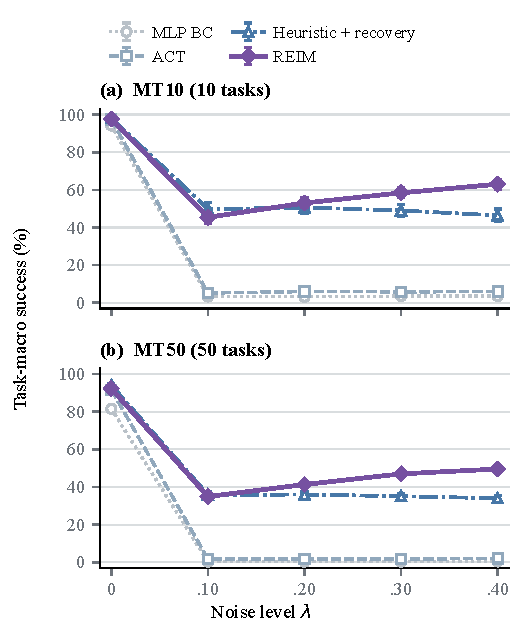
\includegraphics[width=\textwidth]{Figure2_multitask_robustness.pdf}
  \caption{Task-macro success across the shared MT10/MT50 perturbation sweep. Error bars are 95\% within-task bootstrap intervals over 50 episodes per task. Perturbed conditions are a non-official robustness extension.}
  \label{fig:robustness}
\end{figure*}

\subsection{Strong Perturbations: Net Gains with Two-Sided Effects}
Figure~\ref{fig:strong} expands the strongest tested condition. REIM reaches 63.0\% [60.2, 65.6] on MT10 and 49.52\% [48.16, 50.92] on MT50. The heuristic gate reaches 46.4\% [43.2, 49.8] and 33.96\% [32.52, 35.44]. The common recovery policy is therefore not sufficient to explain the difference; how recovery is invoked matters.

The paired decomposition reveals both benefit and harm. On MT10, REIM rescues 115 of 500 episodes (23.0\%) that the heuristic loses, while harming 32 (6.4\%) that the heuristic solves, for a net gain of 16.6 points. On MT50, it rescues 610 of 2,500 episodes (24.4\%) and harms 221 (8.84\%), for a net gain of 15.56 points. Reporting only aggregate success would hide these adverse switches. It would also hide control cost: at $\noise=0.40$, REIM intervenes in 93.4\% of MT10 and 98.68\% of MT50 episodes, with mean recovery occupancies of 69.21\% and 67.40\%, respectively.

\begin{figure*}[t]
  \centering
  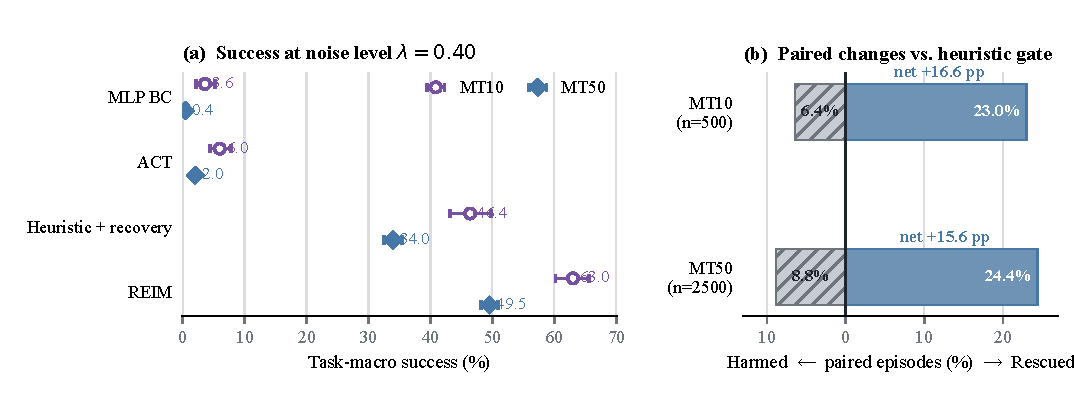
\includegraphics[width=\textwidth]{Figure3_paired_effects.pdf}
  \caption{Results at $\noise=0.40$. (a) Task-macro success with 95\% bootstrap intervals. (b) Paired REIM outcomes relative to heuristic-gated recovery; rescued and harmed are normalized by the suite episode count.}
  \label{fig:strong}
\end{figure*}

\subsection{Benefits Vary Across Task Families}
Figure~\ref{fig:per-task} compares the learned and heuristic gates per task. REIM improves 7 of 10 MT10 tasks and 32 of 50 MT50 tasks, ties on 3 MT50 tasks, and is worse on the remaining 3 and 15 tasks. Both shared and MT50-specific task families appear on either side of the diagonal. The improvement therefore does not arise from one small subset of tasks, but neither is it universal.

The largest positive differences are highly structured. Door-open improves by 82 points in both suites; button-press-topdown improves by 34 points on MT10 and 72 on MT50; and window-close improves by 34 and 70 points. Conversely, MT10 drawer-close and push decline by 14 and 10 points, while MT50 stick-push, coffee-pull, and coffee-push decline by 50, 28, and 26 points. The repeated gains on task families present in both suites support the cross-suite consistency of the learned trigger. The large negative MT50 cases also show why a suite mean cannot substitute for task-level reporting.

The negative cases are consistent with two failure modes. First, a moderate-precision detector may trigger recovery in a state where the nominal chunk would have completed the task. Second, the task-conditioned recovery MLP may not represent every contact mode equally well, especially when the perturbation changes the state faster than the successful continuation data. These interpretations are hypotheses supported by the paired pattern, not separately identified causal effects.

\begin{figure*}[t]
  \centering
  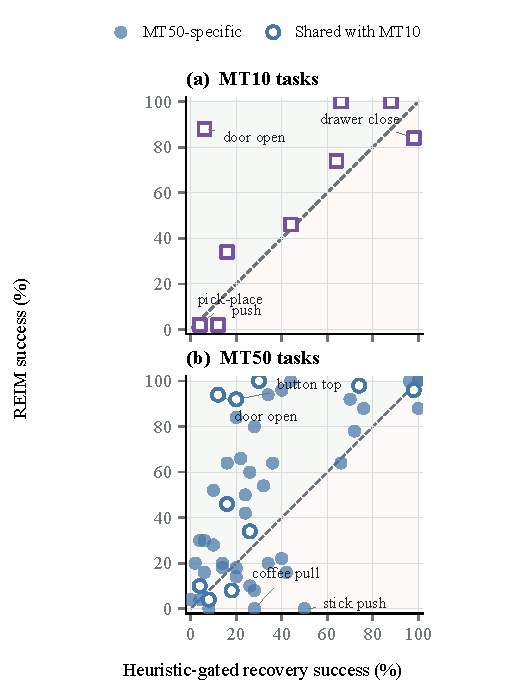
\includegraphics[width=0.88\textwidth]{Figure4_per_task_analysis.pdf}
  \caption{Per-task REIM versus heuristic-gated recovery at $\noise=0.40$. Each point is a 50-episode task mean; points above the diagonal favor REIM. Hollow MT50 markers denote task families shared with MT10.}
  \label{fig:per-task}
\end{figure*}

\subsection{Component Training-Seed Stability}
We additionally vary the detector and recovery optimization seed while keeping the ACT checkpoint fixed. The MT10 study uses seeds 42--44 on its independent 50-episode-per-task bank. The MT50 study uses seeds 42--45 on the main confirmation bank; its recovery-collection bank and deployment threshold are fixed. For each MT50 seed, REIM and the heuristic gate use the same seed-specific recovery checkpoint, so their difference isolates arbitration at deployment. Table~\ref{tab:seeds} reports means and sample standard deviations without pooling the two study banks. Under $\noise=0.40$, all four MT50 REIM seeds reach 47.24--49.52\% success, while their matched heuristic controllers reach 33.96--36.00\%; the paired advantage is 12.52--15.56 points (mean 13.65). At $\noise=0.10$, however, MT50 seed variation is larger and every REIM seed remains below its matched heuristic, reinforcing that the learned gate is not advantageous at the lightest perturbation.

\begin{table}[!b]
\centering
\caption{Component training-seed stability: task-macro success (\%).}
\label{tab:seeds}
\footnotesize
\setlength{\tabcolsep}{3.0pt}
\begin{tabular}{llcc}
\toprule
Suite & $\noise$ & REIM & Heuristic \\
\midrule
MT10 (3 seeds) & 0 & $96.6\pm0.4$ & $96.7\pm0.9$ \\
 & 0.10 & $44.1\pm1.3$ & $44.7\pm3.2$ \\
 & 0.40 & $60.8\pm4.9$ & $40.8\pm3.6$ \\
\midrule
MT50 (4 seeds) & 0 & $92.36\pm0.35$ & $93.46\pm0.62$ \\
 & 0.10 & $34.39\pm2.59$ & $37.38\pm1.31$ \\
 & 0.40 & $48.75\pm1.05$ & $35.10\pm0.94$ \\
\bottomrule
\end{tabular}
\end{table}

\section{Discussion and Limitations}
\label{sec:discussion}

The experiments separate three questions. First, recovery can restore performance after both nominal policies collapse under the tested perturbations. Second, learned risk arbitration becomes more useful than reward stagnation as disturbance strength increases. Third, this advantage is not free: false or mistimed interventions harm some paired episodes, and recovery occupancy is high at strong perturbations. REIM should therefore be interpreted as a robustness mechanism, not an efficiency improvement.

The detector thresholds of 0.65 and 0.64 are independently selected suite operating points, not evidence leakage. Selection uses only the validation bank and a common precision constraint, after which the values are frozen for confirmation evaluation. Their closeness is incidental. Task-macro precision just above 0.60 is modest, and ECE around 0.14 indicates imperfect calibration. Hysteresis and the downstream recovery policy make the risk score operationally useful, but they do not convert it into a calibrated probability of final failure.

Several limits bound the conclusions. All quantitative experiments are in Meta-World simulation and use known task identities; no unseen-task or real-robot transfer is tested. MT10 and MT50 use separately trained models, so cross-suite comparisons describe reproducibility of the pattern rather than a single model scaling from 10 to 50 tasks. The robustness sweep adds i.i.d. Gaussian state and action noise and does not cover camera occlusion, dynamics shift, object relocation, or adversarial disturbances. The PickPlace sequence in Fig.~\ref{fig:overview}(a) is a single qualitative example under a separate single-task protocol and is not part of the MT10/MT50 aggregate comparison. Finally, successful expert continuations may underrepresent unrecoverable or contact-rich states, and the high recovery occupancy suggests that future work should optimize success jointly with intervention burden.

Three follow-up experiments would directly test the present interpretation. First, matching REIM and the heuristic gate by recovery occupancy would separate trigger quality from additional control effort. Second, adding structured disturbances at controlled times would reveal whether the detector responds to causal state changes or merely to generic off-manifold observations. Third, a held-out-task protocol with a task representation other than one-hot identity would test whether the learned notion of risk transfers across task families. These are proposed tests, not claims supported by the current data.

\section{Conclusion}
\label{sec:conclusion}

REIM combines action-chunking imitation, causal near-term risk monitoring, supervised recovery, and hysteretic arbitration in one multi-task manipulation controller. Across matched MT10 and MT50 perturbation sweeps, it preserves clean performance and improves strong-noise success over both nominal policies and a heuristic gate using the same recovery controller. Paired and per-task analyses show why an aggregate gain is not the whole story: interventions both rescue and harm episodes, and their effect varies by task. The next empirical step is to reduce unnecessary intervention while testing structured disturbances and real-robot execution.

\section*{Reproducibility and Disclosure}
The repository records task-bank fingerprints, checkpoint hashes, paired episode identifiers, and figure-generation scripts. \todo{insert public code/data URL or an anonymized artifact statement}. \todo{insert funding and conflict-of-interest statements}. \todo{confirm the target IEEE conference policy and add any required generative-AI disclosure}. Human authors must verify all claims, citations, and final formatting before submission.

\bibliographystyle{IEEEtran}
\IEEEtriggeratref{3}
\bibliography{../paper_assets/reim_refs}

\end{document}
